Aby pokazać ideę testów jednostkowych wykorzystamy model Event, główny trzon aplikacji.

Zaczynamy od wskazania klasy, która będzie testowana. Typ nie jest obowiązkowy, ale RSpec daje nam kilka predefiniowanych typów, m.in. \emph{controller}, \emph{model} czy \emph{routing} z czego warto korzystać. Oczywiście można testować też klasy, które nie należą do żadnego, ale korzystanie z nich znacznie przyspiesza wykonywanie testów.

\begin{code}
	\lstinputlisting[linerange={3-4}, firstnumber=1]{../meetspace/spec/models/event_spec.rb}
\end{code}\\

W drugiej linijce zadeklarowana jest zmienna \emph{event}, która przechowuje obiekt opisywanej klasy. RSpec wykorzystuje tzw. leniwe deklarowanie (\emph{lazy loading}). Zmienna, w tym przypadku obiekt, jest tworzona w momencie natrafienia na nią podczas wykonywania pliku.

\begin{code}
	\lstinputlisting[linerange={41-49}, firstnumber=3]{../meetspace/spec/models/event_spec.rb}
\end{code}\\

Słowo ,,\emph{Describe}'' służy do tworzenia osobnego bloku, co zwiększa czytelność i pozwala szybko zorientować się w pliku. Opisy bloków i testów są o tyle ważne, że tworzą swoistego rodzaju dokumentację. Na pierwszy rzut oka widać jakie testy znajdują się w bloku i co one testują.

W tym przykładzie sprawdzana jest asocjacja między obiektem klasy \emph{User} a wydarzeniem. Chcemy aby jedno wydarzenie należało do jednego użytkownika, dlatego deklarujemy zmienną \emph{user}, która jest instancją\footnote{Obiekt stworzony na podstawie danej klasy.} klasy \emph{User}. Następnie do pola \emph{user\_id} obiektu \emph{event} przypisujemy numer identyfikacyjny(id) obiektu \emph{user}.

\begin{code}
	\lstinputlisting[linerange={43-44}, firstnumber=5]{../meetspace/spec/models/event_spec.rb}
\end{code}\\

Na koniec oczekujemy, że obiekt \emph{event} będzie \emph{,,należał do''} obiektu \emph{user}, oraz, że w polu \emph{event.user} będzie dokładnie ten sam, zadeklarowany kilka linijek wyżej, obiekt.

\begin{code}
	\lstinputlisting[linerange={46-47}, firstnumber=8]{../meetspace/spec/models/event_spec.rb}
\end{code}\\

Całość jest napisana w taki sposób, że nawet osoba nie wdrożona w projekt jest w stanie przeczytać i zrozumieć co dany test robi.
\\

W następnym przykładzie będziemy testować czy przy zadanych przez nas warunkach obiekt zostanie poprawnie zapisany w bazie.

\begin{code}
	\lstinputlisting[linerange={51-63, 100-100}, firstnumber=1]{../meetspace/spec/models/event_spec.rb}
\end{code}\\

W pierwszym teście ustawiamy pole \emph{name} jako nil\footnote{Wartość pusta. Jak \emph{null} w JavaScript.} i oczekujemy, że obiekt nie zostanie poprawnie zwalidowany.

Drugi test sprawdza poprawną długość pola \emph{name}, które powinno wynosić nie więcej niż 50 znaków. Dlatego do zmiennej wstawiamy losowy tekst składający się z większej ilości.\\

Te dwa testy stanowią przykład, że można pisać testy, idąc tzw. ,,czerwoną ścieżką'', czyli oczekiwać, że coś się nie powiedzie.

Ponież przedstawiony jest rezultat wszystkich testów jednostkowych.

\begin{figure}[h]
  \centering
  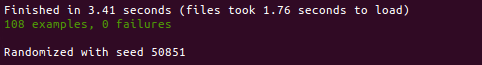
\includegraphics[scale=0.8]{images/rspec_result.png}
  \caption{Wyniki końcowe testów jednostkowych.}
\end{figure}
